\documentclass[a4paper,12pt]{article}
\usepackage{graphicx}
\usepackage{float}
\usepackage[english,russian]{babel}

\title{1.4.1 Изучение физического маятника}
\author{Тимур Байдюсенов Б01-302}
\date{29.09.2023}

\begin{document}
\maketitle

\section{Аннотация}
В работе определяется справедливость формул периода колебаний для физического маятника и значение g. Во время выполнения работы исследовалась зависимость периода колебаний физического маятника от его момента инерции. При обработке результатов оценил погрешность прямых и косвенных измерений.

\section{Теоретические сведения}
Физический маятник - любое твёрдое тело, которое под действием силы тяжести может свободно качатся вокруг неподвижной горизонтальной оси. Движение маятника описывается уравнением:
\begin{equation}
J\frac{d^2\varphi}{dt^2} = M
\end{equation}
где $J$ = момент инерции мятника, $\varphi$ - угол отклонения маятника от положения равновесия, $t$ - время, $M$ - момент сил, действующих на маятник

По теореме Гюйгенса-Штейнера момент инерции маятника вычисляется по формуле:
\begin{equation}
J = \frac{ml^2}{12}+ma^2
\end{equation}

Момент силы тяжести, действующий на маятник:
\begin{equation}
M = -mga\sin\varphi
\end{equation}
При малых углах $\varphi$ формула приобретает вид:
\begin{equation}
M \approx -mga\varphi
\end{equation}

Подставляя выражение для $J$ и $M$ в (1), получаем уравнениие:
\begin{equation}
\ddot{\varphi}+\omega^2\varphi=0
\end{equation}
где 
\begin{equation}
\omega^2 = \frac{ga}{a^2 + \frac{l^2}{12}}
\end{equation}

Период колебаний находится по формуле:
\begin{equation}
T = \frac{2\pi}{\omega} = 2\pi\sqrt{\frac{a^2 + \frac{l^2}{12}}{ag}}
\end{equation}

Период колебаний маятника без груза находится по формуле:
\begin{equation}
T = 2\pi\sqrt{\frac{\frac{l^2}{12} + a^2}{g(1 + \frac{m_{\mbox{пр}}}{m_{\mbox{ст}}})x_{\mbox{ц}}}}
\end{equation}

Период колебаний маятника с грузом находится по формуле:
\begin{equation}
T = 2\pi\sqrt{\frac{J_0 + m_{\mbox{г}}y^2}{gMx_{\mbox{ц}}}}
\end{equation}

\section{Оборудование}

\begin{figure}[H]
\begin{center}
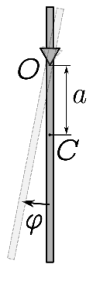
\includegraphics[width=0.2\textwidth]{маятник без груза}
\end{center}
\caption{А: Стержень как физический маятник}
\end{figure}

\begin{figure}[H]
\begin{center}
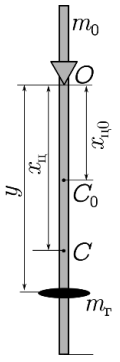
\includegraphics[width=0.2\textwidth]{маятник с грузом}
\end{center}
\caption{Б: Маятник с дополнительным грузом}
\end{figure}

\section{Результаты измерений и обработка данных}


\section{Вывод}
Определил справедливость формул периода колебаний для физического маятника и значение g. Во время выполнения работы исследовалал зависимость периода колебаний физического маятника от его момента инерции. При обработке результатов оценил погрешность прямых и косвенных измерений.

\end{document}
